\section{Performance and Resource Consumption}
\label{sec:comparativeperformance}

In terms of resource consumption, the results observed with GNS3, on one side, and Kathará and CORE, on the other, were very different.
That has an impact in the required computer infrastructures and setups required to do the experiments.

As stated in the explanation between containers-as-lightweight-virtual-machines versus standard \glspl{vm}, a container provides a virtual isolation of the filesystem and networking (among others) for its processes while \glspl{vm} need everything, in every layer of software, a regular host has to run (operating system, libraries, applications) to be loaded each time for each running virtual machine.

In a running Kathará, CORE, or GNS3 topology, there are associated processes to each node.
As previously shown, GNS3's Cisco routers can be \glspl{vm} running the modern Cisco IOSv or processes of the Dynamips emulator which in fact is a virtual machine, but not in the sense of \textquote{a PC running in isolation with virtualized IO} (e.g. the instructions of those IOS images isn't x86, and therefore there has to be a translation to machine instructions).

Table~\ref{tab:comparativeramusage} lists approximate values measured with the \texttt{top} command (and \texttt{docker~stats}, for Kathará's) on more than one GNU/Linux system for the memory consumption of each process that backs a live node in a topology for each studied possibility.
These measures only approximate the order of magnitude, in a sense that can be described as: \textquote{of several different times the values were measured, on more than one machine, they didn't fluctuate more than, say, $50~\mbox{MiB}$ (for GNS3's), $5~\mbox{MiB}$ (for Kathará's), and $1~\mbox{MiB}$ (for CORE's)} and therefore it doesn't correspond to an accurate arithmetic mean or other formal statistical method.

% Table tab:comparativeramusage
\begin{table}
  \centering
  \small
  \begin{tabulary}{0.9\textwidth}{ll}
    \toprule
      \textbf{Topology node}                   & \textbf{Memory usage}\\
    \midrule
      GNS3 -- Cisco IOSvL2 (KVM via QEMU)      & $\approx 460~\mbox{MiB}$\\
      GNS3 -- Cisco c3745 (Dynamips process)   & $\approx 270~\mbox{MiB}$\\
      Kathará (any node is a Docker container) & $\approx 4~\mbox{MiB}$\\
    \bottomrule
  \end{tabulary}
  \caption{%
    Approximate metrics of the memory footprint of (networking) nodes in topologies for different emulators
  }
  \label{tab:comparativeramusage}
\end{table}


For the sake of example, the query for the memory footprint of the running Docker containers on a host (in this case, all of them are Quagga-enabled Linux hosts as Kathará nodes) is shown in figure~\ref{fig:comparative-docker-stats}.

CORE's measure of (idle) memory footprint for a sample router was made summing the memory footprint of an instance of the container launcher process (\texttt{vnoded}), \texttt{ospf6d}, \texttt{ospf}, and \texttt{zebra}.

% Figure fig:comparative-docker-stats
\begin{figure}
  \centering
  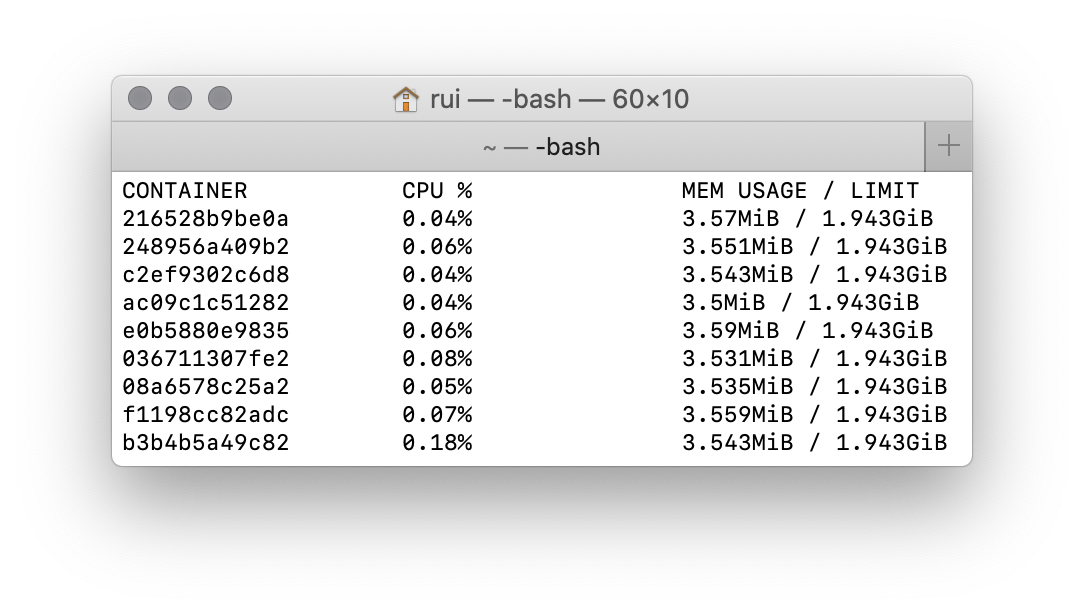
\includegraphics[width=0.8\textwidth]{comparative-docker-stats}
  \caption{The \texttt{docker stats} command showing the resources taken by containers corresponding to nodes in a Kathará lab}
  \label{fig:comparative-docker-stats}
\end{figure}


% end of section comparativeperformance
